\section{Theoretical Analysis}
\label{sec:theoretical_analysis}

This section is broken into three parts. First, we provide a strong lower bound on slack to complete the definition of LVI. Second, we prove convergence given an important assumption, and explain why the assumption must exist. Third, we show two properties of LMDPs: game theory connection and its optimal policy's distinctness with respect to scalarization methods.


\subsection{Strong Bound on Slack}

First we show in Proposition~\ref{prop:lvi_eta} proves that $\eta_i$ from Equation~\ref{eq:restricted_actions_set} may be defined as $(1 - \gamma) \delta_i$ to bound the final deviation from the optimal value of a state by $\delta_i$, for $i \in K$. This is designed to be a worst-case guarantee that considers each state selects an action as far from optimal as it can, given the slack allocated to it. The accumulation of error over all states is bounded by $\delta$. In practice, this strong lower bound constraint can be relaxed, if desired.


\begin{proposition}
    \label{prop:lvi_eta}
    For all $j \in L$, for $i \in K$, assume $1, \ldots, i - 1$ has converged. Let $V^\eta$ be the value functions returned following Equation~\ref{eq:lvi}; Lines 7-10. Let $V^\pi$ be the value functions returned by value iteration, following the resulting optimal policy $\pi$, starting at $V^\eta$. If $\eta_i = (1 - \gamma) \delta_i$ then $\forall s \in S_j$, $V_i^\eta(s) - V_i^\pi(s) \leq \delta_i$.
\end{proposition}

\begin{proof}
For any $i \in K$, the full (infinite) expansion of value iteration for $V_i^\eta$ is as follows ($t \rightarrow \infty$).
\begin{align}
    V_i^\pi(s) &= \sum_{s^t \in S} T(s, \pi(s), s^t) \Big( R_i(s, \pi(s), s^t) + \gamma \Big( \cdots \nonumber \\
        &+ \gamma \Big( \sum_{s^1 \in S} T(s^2, \pi(s^2), s^1) \Big( R_i(s^2, \pi(s^2), s^1) \label{eq:lvi_eta_1} \\
        &+ \gamma \Big( V_i^0 (s^1) \Big) \Big) \Big) \cdots \Big) \Big) \label{eq:lvi_eta_2}
\end{align}

Since value iteration admits exactly one unique fixed point, any initial value of $V_i^0$ is allowed; we let $V_i^0 = V_i^\eta$. From this, $Q_i^\eta(s, \pi(s))$ (Equation~\ref{eq:value_of_state_action}) exists within lines~\ref{eq:lvi_eta_1} and~\ref{eq:lvi_eta_2}. Also, by Equation~\ref{eq:restricted_actions_set}, $V_i^\eta(s) - Q_i^\eta(s, \pi(s)) \leq \eta_i$ since $\pi(s) \in A_k(s) \subseteq \cdots \subseteq A_{i+1}(s)$. Equivalently, $Q_i^\eta(s, \pi(s)) \geq V_i^\eta(s) - \eta_i$. Combine all of these facts and bound it from below.
\begin{align*}
    V_i^\pi(s) &\geq \sum_{s^t \in S} T(s, \pi(s), s^t) \Big( R_i(s, \pi(s), s^t) + \gamma \Big( \cdots \nonumber \\
        &+ \gamma \Big( \sum_{s^2 \in S} T(s^3, \pi(s^3), s^2) \Big( R_i(s^3, \pi(s^3), s^2) \\
        &+ \gamma \Big( V_i^\eta(s^2) - \eta_i \Big) \Big) \Big) \cdots \Big) \Big)
\end{align*}

The $\eta_i$ falls out of the inner equation. Also, recall that $\sum_{s^2 \in S} T(s^3, \pi(s^3), s^2) = 1$ and $\gamma \eta_i$ is a constant.
\begin{align*}
        &\geq \sum_{s^t \in S} T(s, \pi(s), s^t) \Big( R_i(s, \pi(s), s^t) + \gamma \Big( \cdots \\
        &+ \gamma \Big( \sum_{s^2 \in S} T(s^3, \pi(s^3), s^2) \Big( R_i(s^3, \pi(s^3), s^2) \\
        &+ \gamma \Big( V_i^\eta(s^2) \Big) \Big) - \gamma \eta_i \Big) \cdots \Big) \Big)
\end{align*}

We may again recognize the existence of $Q_i^\eta(s^3, \pi(s^3))$ and place a lower bound on the next one with $V_i^\eta(s^3) - \eta_i$. This process repeats, each time introducing a new $\eta_i$, with one less $\gamma$ multiplied in front of it, until we reach the final equation. We obtain the following inequality, and note that if $\eta_i \geq 0$, then we may subtract another $\eta_i$ in order to obtain a geometric series (i.e., the sum may begin at $t = 0$).
\begin{equation*}
    V_i^\pi(s) \geq V_i^\eta(s) - \sum_{t = 0}^\infty \gamma^t \eta_i \geq V_i^\eta(s) - \frac{\eta_i}{1 - \gamma}
\end{equation*}
\begin{equation*}
    V_i^\eta(s) - V_i^\pi(s) \leq \frac{\eta_i}{1 - \gamma}
\end{equation*}

Therefore, let $\eta_i = (1 - \gamma) \delta_i$. This guarantees that error \emph{for all} states $s \in S$ is bounded by $\delta_i$.
\end{proof}


\subsection{Convergence Properties}

In order to prove convergence of Algorithm~\ref{alg:lvi}, we must first prove Proposition~\ref{prop:lvi_contraction}. It states that the value iteration component over a state partition with slack is a contraction map. The proof itself follows from value iteration~\cite{Bellman57} and from the suggested proof by Russel and Norvig~\shortcite{Russell10-AI}. We include it here since there are a few modifications required (restricted actions and fixed values), and it explains exactly why we must make an assumption about convergence of LVI.


\begin{proposition}
    \label{prop:lvi_contraction}
    For all $j \in L$, for $i \in K$, assume $1, \ldots, i - 1$ has converged, with discount factor $\gamma \in [0, 1)$. $B_i$ (Equation~\ref{eq:lvi}) is a contraction map in the space of value functions over $s \in S_j$, i.e., $\| B_i V_1 - B_i V_2 \|_\infty^{S_j} \leq \gamma \| V_1 - V_2 \|_\infty^{S_j}$.
\end{proposition}

\begin{proof}
For a metric space $\langle Y, d \rangle$, where $Y$ is a set and $d$ is a distance metric, a map $f : Y \rightarrow Y$ is called a \emph{contraction map} if there exists an $\alpha$ such that $d(f(x), f(y)) = \alpha d(x, y)$, for all $x, y \in Y$.

Let the space $Y_i = \mathbb{R}^z$ be the \emph{space of value functions for $i$} for $z = |S_j|$, i.e., we have $V_i = [V_i(s_{j1}), \ldots, V_i(s_{jz})]^T \in Y_i$. Let the distance metric $d_i$ be the \emph{max norm}, i.e., $\|V_i\|_\infty = \max_{s \in S_j} |V_i(s)|$. Since $\gamma \in [0, 1)$, the metric space $M_i = \langle Y_i, d_i \rangle$ is a \emph{complete normed metric space} (i.e., \emph{Banach space}). %; every Cauchy sequence of $M_i$ converges to a point in $M_i$.

Let the lexicographic Bellman optimality equation for $i$ (Equation~\ref{eq:lvi}) be defined as an operator $B_i$. Must show the operator $B_i$ is a contraction map in $M_i$ for all $i \in K$, given either that $i=1$ or that the previous $i-1$ has converged to within $\epsilon$ of its fixed point.

Let $V_1, V_2 \in Y_i$ be any two value function vectors. Apply Equation~\ref{eq:lvi}. For $s \in S_j$, if $i = 1$ then $A_i(s) = A$; otherwise, $A_i(s)$ is defined using $A_{i-1}(s)$ (Equation~\ref{eq:restricted_actions_set}) which by construction have converged.
\begin{equation*}
    \| B_i V_1 - B_i V_2 \|_\infty^{S_j} = \max_{s \in S_j} | \max_{a \in A_i(s)} Q_1(s, a) - \max_{a \in A_i(s)} Q_2(s, a) |
\end{equation*}

As part of the $Q(\cdot)$ values, we distribute $T(\cdot)$ to each $R(\cdot)$ and $V(\cdot)$ in the summations, then apply the property: $\max_x f(x) + g(x) \leq \max_x f(x) + \max_x g(x)$, twice.
\begin{align*}
%    &\| B_i V_1 - B_i V_2 \|_\infty^{S_j} \\
    &\leq \max_{s \in S_j} \Big| \max_{a \in A_i(s)} \Big( \sum_{s' \in S} T(s, a, s') R_i(s, a, s') \\
    &\quad \quad + \gamma \sum_{s' \in S} T(s, a, s') \bar{V}_1(s') \Big) \\
    &\quad \quad - \max_{a \in A_i(s)} \Big( \sum_{s' \in S} T(s, a, s') R_i(s, a, s') \\
    &\quad \quad - \gamma \sum_{s' \in S} T(s, a, s') \bar{V}_2(s') \Big) \Big| \\
    &\leq \max_{s \in S_j} \Big| \gamma \max_{a \in A_i(s)} \sum_{s' \in S} T(s, a, s') \bar{V}_1(s') \\
    &\quad \quad - \gamma \max_{a \in A_i(s)} \sum_{s' \in S} T(s, a, s') \bar{V}_2(s') \Big|
\end{align*}

First, we can pull out $\gamma$. Recall, also that for any two functions $f$ and $g$, $| \max_x f(x) - \max_x g(x) | \leq \max_x | f(x) - g(x) |$. %After applying this property, we note that $T(\cdot)$ lies on an $n$-simplex, which forms a simple convex polytope after scaling the value function difference. Convex polytopes obtain their maximum values at the vertices, allowing us to select the maximal state $s \in S$ instead.
\begin{align*}
%    &\| B_i V_1 - B_i V_2 \|_\infty^{S_j} \\
%    &\leq \gamma \max_{s \in S_j} \max_{a \in A_i(s)} \Big| \sum_{s' \in S} T(s, a, s') (\bar{V}_1(s') - \bar{V}_2(s')) \Big| \\
    &\leq \gamma \max_{s \in S_j} \max_{a \in A_i(s)} \sum_{s' \in S} T(s, a, s') \Big| \bar{V}_1(s') - \bar{V}_2(s') \Big|
\end{align*}

Now, we can apply Equation~\ref{eq:lvi_V_bar}. Note the {\bf requirement} that $\| V_1^{fixed} - V_2^{fixed} \|_\infty^{S \setminus S_j} \leq \| V_1 - V_2 \|_\infty^{S_j}$. With this assumption, we will be left with the difference of $V_1$ and $V_2$ over $S_j$, and thus a contraction map.
\begin{align*}
    &\leq \gamma \max_{s \in S_j} \max_{a \in A_i(s)} \sum_{s' \in S_j} T(s, a, s') \Big| V_1(s') - V_2(s') \Big| \\
    &\leq \gamma \max_{s \in S_j} \Big| V_1(s) - V_2(s) \Big| \\
    &\leq \gamma \| V_1 - V_2 \|_\infty^{S_j}
\end{align*}
This proves that the operator $B_i$ is a contraction map on metric space $M_i$, for all $i \in K$.
\end{proof}


Following the same logic as Bellman's optimality equation, we may guarantee convergence to within $\epsilon > 0$ of the fixed point (Proposition~\ref{prop:lvi_convergence}). We omit this proof, since it follows exactly like previous proofs and, unlike Proposition~\ref{prop:lvi_contraction}, there are no important components which affect further results. The full proof is provided in the supplementary material for the sake of completeness.


\begin{proposition}
    \label{prop:lvi_convergence}
    For all $j \in L$, for $i \in K$, assume $1, \ldots, i - 1$ has converged. Following Equation~\ref{eq:lvi}; Lines 7-10, for any $i \in K$, $B_i$ converges to within $\epsilon > 0$ of a unique fixed point once $\| V_i^{t+1} - V_i^t \|_\infty^{S_j} < \epsilon \frac{1 - \gamma}{\gamma}$ for iteration $t > 0$.
\end{proposition}


As we found in Proposition~\ref{prop:lvi_contraction}'s proof, there is an implicit constraint underlying its application. Proposition~\ref{prop:lvi_convergence} leverages \emph{Banach's fixed point theorem}, which itself proves convergence by constructing a sequence of value functions in the metric space, following the contraction operator. This is trivially true for the inner while loop on Lines 8-11, but not necessarily true for the outer while loop.

For convergence proof we use Banach's fixed point theorem to ensure uniqueness. Therefore, we must assume a bound on the difference between $V^{fixed}$ over each iteration (Assumption~\ref{ampt:proper_partitions}). Intuitively, with respect to LVI, the assumption takes whichever partition is the source of the largest error, and assumes that it always the source of the largest error until it converges. We prove that LVI converges to a unique fixed point under this assumption in Proposition~\ref{prop:lvi}.


\begin{assumption}[Proper Partitions]
    \label{ampt:proper_partitions}
    Let $j \in L$ be the partition which satisfies $\| V_1^{fixed} - V_2^{fixed} \|_\infty^{S \setminus S_j} \leq \| V_1 - V_2 \|_\infty^{S_j}$ from Proposition~\ref{prop:lvi_contraction}. Let $i \in K$ such that $1, \ldots, i - 1$ has converged. Assume that this inequality holds until $j$ has converged to within $\epsilon$, and that it remains fixed at $V_i^{fixed}$.
    % $\| B_i V_i^{fixed} - V_i^{fixed} \|_\infty^{S \setminus S_j} \leq \| B_i V_i - V_i \|_\infty^{S_j}$
\end{assumption}


\begin{proposition}
    \label{prop:lvi}
    LVI (Algorithm~\ref{alg:lvi}) converges to a unique fixed point $V^*$ under Assumption~\ref{ampt:proper_partitions} with $\gamma \in [0, 1)$.
\end{proposition}


\begin{proof}
Must show that for each partition, all value functions converge following the respective orderings, in sequence, to a unique fixed point. We do this by constructing a metric space of the currently converged values, and the ones that are ``converging'' (i.e., satisfying Assumption~\ref{ampt:proper_partitions}). Then, we apply Proposition~\ref{prop:lvi_contraction} which proves that $G$ is a contraction map on this space. Finally, since this is true for all partitions and their value functions, and Assumption~\ref{ampt:proper_partitions} guarantees converged values remain stable, it converges to the entire metric space over the entire partitions and their values.

Let $Y$ be the space of all value functions over partitions $\forall j \in L' \subseteq L$, value functions $K_j' \subseteq K$, and their states $S$ which have converged or satisfy Assumption~\ref{ampt:proper_partitions}. Note that the base case includes only the first $o_j(1) \in K_j'$ from each $j \in L'$. Let distance metric $d$ be the \emph{max norm}, i.e., $\|V\|_\infty$ $=$ $\max_{j \in L'} \max_{i \in K_j'} \max_{s \in S_j} | V_i(s) |$. Thus, the metric space $M = \langle Y, d \rangle$ is a \emph{Banach space}.

Let $G$ be an operator in $M$ following Lines 4-13 in Algorithm~\ref{alg:lvi}, i.e., $V' = GV$ using the algorithm's variables: $V$ and $V'$. Must show that $G$ is a contraction map. Let $V_1, V_2 \in Y$ be any two value function vectors. Rewrite in terms of $B_i$ and then apply Proposition~\ref{prop:lvi_contraction}.
\begin{align*}
    \| G V_1 - G V_2 \|_\infty &= \max_{j \in L'} \max_{i \in K_j'} \max_{s \in S_j} | (G V_1)_i (s) - (G V_2)_i (s) | \\
        &= \max_{j \in L'} \max_{i \in K_j'} \max_{s \in S_j} | B_i V_{1i} (s) - B_i V_{2i} (s) | \\
        &\leq \gamma \max_{j \in L'} \max_{i \in K_j'} \max_{s \in S_j} | V_{1i} (s) - V_{2i} (s) | \\
        &\leq \gamma \| V_1 - V_2 \|_\infty
\end{align*}

Therefore, $G$ is a contraction map. By \emph{Banach's fixed point theorem}, since $M$ is a complete metric space and $G$ is a contraction map on $Y$, $G$ admits a unique fixed point $V^* \in Y$.

By Assumption~\ref{ampt:proper_partitions}, for any initial configuration, it converges to a unique fixed point, which produces a new metric space, which converges to a new unique fixed point, etc. This process repeats to completion until we reach the entire space over $\mathbb{R}^{\ell \times k \times n}$, yielding a final unique fixed point $V^*$.
\end{proof}


\subsection{Relation to Other Models}

Interestingly, there is a connection between LMDPs and game theory; specifically, Definition~\ref{def:lmdp_normal_form} describes a mapping from an LMDP to a \emph{normal form game}. Intuitively, each partition can be thought of as a player in a game. The action a partition can take are any sub-policy for the states in the partition. We select any $\ell$ value functions, one from each partition, and use those as the payoffs for a normal form game. We show in Proposition~\ref{prop:lvi_nash} that the resulting LMDP's optimal policy computed from LVI is, in fact, a Nash equilibrium.


\begin{definition}
    \label{def:lmdp_normal_form}
    Let LMDP $\langle S, A, T, \mathbf{R}, \delta, \mathcal{S}, o \rangle$ have value functions $V^\pi$ for corresponding optimal policy $\pi$, the optimal value functions $V^\eta$, computed via LVI (Algorithm~\ref{alg:lvi}). Let $\bar{s} = \langle s_1, \ldots, s_\ell \rangle$ be a state tuple such that $\forall z \in L$, $s_z \in S_z$. Let $\bar{i} = \langle i_1, \ldots, i_\ell \rangle$ be any tuple of indices $i_z \in K$.

    The \textbf{LMDP's Normal Form Game} $\langle L, \mathcal{A}, U \rangle$ is:
    \begin{itemize}
        \item $L = \{1, \ldots, \ell\}$ is a set of agents (partitions)
        \item $\mathcal{A} = \mathcal{A}_1 \times \cdots \times \mathcal{A}_\ell$ is a finite set of joint actions, such that $\forall z \in L$, $x = |S_z|$, $S_z = \{s_{z1}, \ldots, s_{zx}\}$, $\mathcal{A}_z = A_{i_z}(s_{z1}) \times \cdots \times A_{i_z}(s_{zx})$
        \item $U = \langle u_1, \ldots, u_\ell \rangle$ is a set of utility functions, such that $\forall z \in L$, $\forall a \in \mathcal{A}$, $s_z \in \bar{s}$, $u_z(a_z, a_{-z}) = \min \{ V_{i_z}^{\pi, a_z} (s_z), V_{i_z}^\eta (s_z) - \delta_{i_z} \}$.
    \end{itemize}
\end{definition}

Note that we only consider pure strategy profiles. Thus, a player's \emph{strategy set} will be used synonymously with its \emph{action set}. Similarly, since we consider one stage games, \emph{strategy profile} will be synonymous with \emph{action profile}.


\begin{proposition}
    \label{prop:lvi_nash}
    For LMDP $\langle S, A, T, \mathbf{R}, \delta, \mathcal{S}, o \rangle$, let $\pi$ be the optimal policy computed using LVI (Algorithm~\ref{alg:lvi}). Let $f(\pi) = \langle \omega_1, \ldots, \omega_\ell \rangle$ so that $\forall z \in L$, $x = |S_z|$, $S_z = \{ s_{z1}, \ldots, s_{zx} \}$, $\omega_z = \langle \pi(s_{z1}), \ldots, \pi(s_{zx}) \rangle$. Applying the transformation in Definition~\ref{def:lmdp_normal_form}, the strategy (action) profile $f(\pi) = a = (a_z, a_{-z}) \in \mathcal{A}$ is a weak pure strategy Nash equilibrium.
\end{proposition}

\begin{proof}
By the definition of a (weak) Nash equilibrium, must show that $\forall z \in L$, $\forall a' \in \mathcal{A}_z$, $u_z(a_z, a_{-z}) \geq u_z(a', a_{-z})$.

Let $\pi'$ be the corresponding policy for $f(\pi')$ $=$ $\langle a_1, \ldots, a_{z-1}, a', a_{z+1}, \ldots, a_\ell \rangle$ $\in \mathcal{A}$. Recall that $a' = \langle a_1', \ldots, a_x' \rangle$, $x = |S_z|$.

Let $V^{\pi'}$ be the value functions after value iteration has converged for each value function in $K$ following policy $\pi'$. Note that $\mathbf{V}_x^\pi = \mathbf{V}_x^{\pi'}$, $\forall x \in \{1, \ldots, i_z - 1\}$, and therefore by Equation~\ref{eq:restricted_actions_set}, $A_{i_z}^\pi = A_{i_z}^{\pi'}$. This ensures that we may use Proposition~\ref{prop:lvi_eta}, by simply considering a MOMDP with a reduced number of rewards up to $i_z$.

By Proposition~\ref{prop:lvi_eta}, $V_{i_z}^\pi (s_z) \geq V_{i_z}^\eta (s_z) - \delta_i$. Apply the fact that $\pi$ is defined following action $a_z$, so $V_{i_z}^{\pi, a_z} (s_z) = V_{i_z}^\pi (s_z)$. Thus, by Definition~\ref{def:lmdp_normal_form}:
\begin{equation*}
    u_z(a_z, a_{-z}) = \min \{ V_{i_z}^\pi (s_z), V_{i_z}^\eta (s_z) - \delta_i \} = V_{i_z}^\eta (s_z) - \delta_i
\end{equation*}
There are two cases for $V_{i_z}^{\pi'} (s_z)$; regardless, the inequality $u_z(a_z, a_{-z}) \geq u_z(a', a_{-z})$ is true. Therefore, the strategy (action) profile $\pi$ is a Nash equilibrium.

%\emph{Case 1:} $V_{i_z}^{\pi'} (s_z) \geq V_{i_z}^\eta (s_z) - \delta_i$. Which implies:
%\begin{equation*}
%    u_z(a', a_{-z}) = \min \{ V_{i_z}^{\pi'} (s_z), V_{i_z}^\eta (s_z) - \delta_i \} = V_{i_z}^\eta (s_z) - \delta_i
%\end{equation*}
%Therefore, $u_z(a_z, a_{-z}) = u_z(a', a_{-z})$.
%
%\emph{Case 2:} $V_{i_z}^{\pi'} (s_z) < V_{i_z}^\eta (s_z) - \delta_i$. Which implies:
%\begin{equation*}
%    u_z(a', a_{-z}) = \min \{ V_{i_z}^{\pi'} (s_z), V_{i_z}^\eta (s_z) - \delta_i \} = V_{i_z}^{\pi'} (s_z)
%\end{equation*}
%Therefore, $u_z(a_z, a_{-z}) > u_z(a', a_{-z})$.

%In both cases, the inequality $u_z(a_z, a_{-z}) \geq u_z(a', a_{-z})$ is true. Therefore, the strategy (action) profile $\pi$ is a Nash equilibrium.

\end{proof}

So far, we have shown some convergence properties of LVI and a connection to game theory. We will now prove a uniqueness property in relation of linearly weighted scalarization functions; in particular, there exist LMDPs such that for the corresponding MOMDP, no weight exists which would allow VI to return the same policy as LVI. The idea is to construct a MOMDP which has conflicting weight requirements to produce the policy returned by LVI.


\begin{figure}% [H]
\begin{center}
    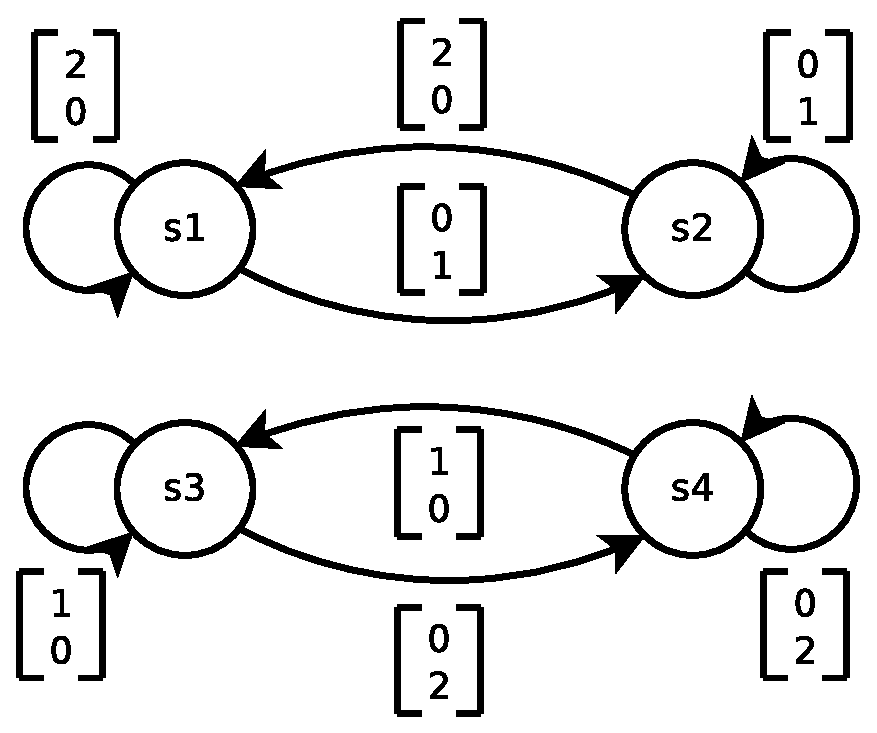
\includegraphics[width=0.75\linewidth]{momdp.eps}
    \caption{The example MOMDP for Proposition~\ref{prop:lvi_uniqueness}.}
    \label{fig:example_momdp}
\end{center}
\end{figure}


\begin{proposition}
    \label{prop:lvi_uniqueness}
    There exist LMDPs, with a policy following LVI $\pi$, such that for all weights $\mathbf{w}$, the corresponding scalarized MOMDP's policy $\pi_{\mathbf{w}}$ is not equal to $\pi$.
\end{proposition}

\begin{proof}
Consider the MOMDP depicted in Figure~\ref{fig:example_momdp}, with states $S = \{s_1, s_2, s_3, s_4\}$, $A = \{stay, leave\}$, $T(s, stay, s') = 1$ if $s = s'$, $T(s, leave, s') = 1$ if $s \neq s'$, $T(s, a, s') = 0$ otherwise, and rewards $\mathbf{R} = [ R_1, R_2 ]^T$ as shown.

For states $s_1$ and $s_2$, $w_1 < 1/3$ and $w_2 > 2/3$ produce the policy $\pi_\mathbf{w}(s_1) = leave$ and $\pi_\mathbf{w}(s_2) = stay$. Similarly, weights $w_1 > 1/3$ and $w_2 < 2/3$ produce the policy $\pi_\mathbf{w}(s_1) = stay$ and $\pi_\mathbf{w}(s_2) = leave$. Only weights set to $w_1 = 1/3$ and $w_2 = 2/3$ allows for ambiguity; a carefully selected tie-breaking rule alows for the policy $\pi_\mathbf{w}(s_1) = \pi_\mathbf{w}(s_2) = stay$.

The exact same logic holds for states $s_3$ and $s_4$ with the weights reversed at $w_1 = 2/3$ and $w_2 = 1/3$ to allow a tie-breaking rule to produce $\pi_\mathbf{w}(s_3) = \pi_\mathbf{w}(s_4) = stay$.

Construct the corresponding LMDP with $\mathcal{S} = \{S_1, S_2\}$, $S_1 = \{s_1, s_3\}$, $S_2 = \{s_2, s_4\}$, $o = \langle o_1, o_2 \rangle$, $o_1 = \langle 1, 2 \rangle$, $o_2 = \langle 2, 1 \rangle$, and $\delta = \langle 0, 0, \rangle$. The policy returned by LVI is $\pi(s) = stay$ for all $s \in S$. This policy is unique since it cannot be produced by any selection of weights.
\end{proof}

%This example also demonstrates the practical use of LVI, since the final values of each state are much higher for $\pi$ than they are for any $\pi_\mathbf{w}$.

%As a final note, it is easy to show that Algorithm~\ref{alg:lvi} generalizes value iteration (VI) and other forms of LVI~\cite{Gabor98-MultiObjectiveReinforcementLearning}.

